\section{Modeling and Controlling ATSs - The MPC for ATS and the RCS} 

% ==================///==================///==================///
\begin{frame}{How can the CATSM shortcomings be solved?}
	Three combined approaches
	\vspace{0.5cm}
	\begin{itemize}
		\item Novel linear discrete-time model
		\item Definition of an ad-hoc model predictive control (MPC) 
		\item Adaptive road network optimization using graph transformation systems (GTS)
	\end{itemize}
\end{frame}

% ==================///==================///==================///
\begin{frame}{Novel Model for ATSs}
	Key idea $\rightarrow$ Define AVs speed in function of the number of AVs currently on the street
	\begin{columns}
		\begin{column}{0.4\textwidth}
			\begin{equation*}
				\resizebox{1.3\textwidth}{!}{$
				\begin{aligned}	
					s_{ij}(V_{ij}) &= \begin{cases}
						l_{ij} \quad\quad &\text{if } V_{ij}\in[0,V_{ij}^{th})\\ 
						l_{ij} - b\cdot(V_{ij}^{th}- V_{ij}) \quad\quad &\text{if }V_{ij}\in[V_{ij}^{th}, V_{ij}^{max})\\ 
						0\quad\quad &\text{if }V_{ij} \ge V_{ij}^{max}\\ 
					\end{cases}\\
					\text{with } b  &=  \dfrac{l_{ij}-\epsilon }{ V_{ij}^{th} -  V_{ij}^{max}} \text{ and } \epsilon \in (0,1)
				\end{aligned}
				$}
			\end{equation*}
			$\rightarrow$ Implicitely, a better congestion model
		\end{column}
		\begin{column}{0.4\textwidth}
			\begin{figure}[t]
				\centering
				\resizebox{1.1\textwidth}{!}{
				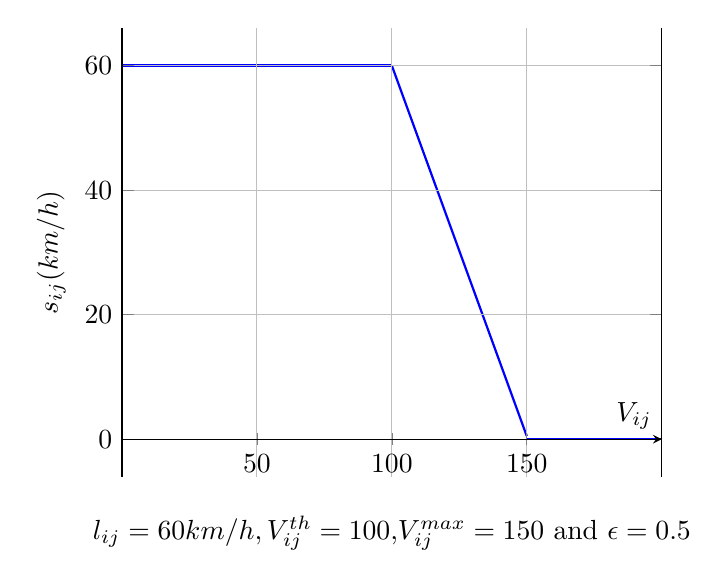
\begin{tikzpicture}
					\begin{axis}[
						xlabel={$V_{ij}$},
						ylabel={$s_{ij} (km/h)$},
						domain=0:250, % adjust the domain based on your preference
						samples=40,
						grid=both,
						axis x line=middle,
						%ymin=-1, % Set the minimum y-axis value
						%ymax=1.4, % Set the maximum y-axis value
						axis on top,
						legend pos=north east,
						title style={at={(0.5,-0.1)},anchor=north,yshift=-0.5},
						title={$l_{ij} = 60 km/h,V_{ij}^{th} = 100$,$V_{ij}^{max} = 150$ and $\epsilon = 0.5$},
						]
						% Piecewise function
						\addplot[blue, thick, domain=0:100] {60};
						\addplot[blue, thick, domain=100:150] {60 - 1.19*(x-100)};
						\addplot[blue, thick, domain=150:200] {0};
						%\addlegendentry{B}
					\end{axis}
				\end{tikzpicture}
			}
			\end{figure}
		\end{column}
	\end{columns}
\end{frame}

% ==================///==================///==================///
\begin{frame}{Novel Model for ATSs}
	As a result, new model linear time-discrete model can be defined, which tracks
	\begin{itemize}
		\item AVs' position using the speed 
		\item Stationed AVs
		\item Served and Unrequests using travelling vehicles
	\end{itemize}
	\vspace{0.3cm}
	$\rightarrow$ It's also easily controllable
\end{frame}

% ==================///==================///==================///
\begin{frame}{MPC for ATSs}
	Let $V_{ij}(t) \in \{ x \in \mathbb{N}_0 : x \leq |\mathcal{A}|\}$ being the total number of vehicles currently circulating on the street $\langle i,j\rangle$, this can be easily computed by adding the number of carries to the rebalancing AVs, i.e. \\
	\begin{equation*}
		V_{ij}(t) = \sum_{a \in \mathcal{A}} v^{a}_{ij}(t) +w^{a}_{ij}(t)
	\end{equation*}
	$\rightarrow$ Control  $v^{a}_{ij}(t)$ and $w^{a}_{ij}(t)$
\end{frame}
% ==================///==================///==================///
\begin{frame}{MPC for ATSs}
	Let $\mathcal{X}$ and $\mathcal{U}$ being the set of feasible states and inputs, respectively, solve
	\begin{equation}
		\begin{aligned}
			\underset{\substack{u(t), \dots, u(t+N)}}{\text{\textbf{min}}} \quad & J_f(x(N))+\sum_{t=0}^{N-1}I(x(t)) \\
			\text{\textbf{s.t.}} \quad & x(t+1) = Ax(t) + Bu(t)  \\
			& x(t) \in \mathcal{X}, \ u(t)\in \mathcal{U} \\
			%& k = t, \dots, t+N\\
			&x(N) \in \mathcal{X}_f\\
		\end{aligned}
	\end{equation}
	where $\mathcal{X}_f$ is the set of terminal states, $J_f(x(N))$ is the terminal cost function and $I(x(t))$ is the stage cost
\end{frame}
% ==================///==================///==================///
\begin{frame}{MPC for ATSs}
The main objectives are to:
\vspace{0.1cm}
\hspace{9.5 cm}\tikzmark{right}
\begin{itemize}
	\item Reduce number of outstanding requests \tikzmark{a}
	\item Minimize unnecessary rebalancing vehicles \tikzmark{b}
	\vspace{0.2cm}
	\item Avoid transportation after requests are served \tikzmark{c}
	\item Avoid rebalancing after requests are served \tikzmark{d}
\end{itemize}
\vspace{0.7cm}
$\rightarrow$ Stability can be proven
\begin{tikzpicture}[overlay, remember picture]
	\node[anchor=base] (1) at (pic cs:a) {\vphantom{h}}; % push the mark to the top of the line (ie including ascenders)
	\node[anchor=base] (2) at (pic cs:b) {\vphantom{g}}; % push the mark to the bottom of the line (ie including descenders)
	\node[anchor=base] (3) at (pic cs:c) {\vphantom{h}}; % push the mark to the top of the line (ie including ascenders)
	\node[anchor=base] (4) at (pic cs:d) {\vphantom{g}}; % push the mark to the bottom of the line (ie including descenders)
	\draw [decoration={brace,amplitude=0.5em},decorate,ultra thick,black]
	(1.north -| {pic cs:right}) -- (2.south -| {pic cs:right}) node[midway, right=1em] {Combined give $I(x(t))$};
	\draw [decoration={brace,amplitude=0.5em},decorate,ultra thick,black]
	(3.north -| {pic cs:right}) -- (4.south -| {pic cs:right}) node[midway, right=1em] {Combined give $J_f(x(N))$};
\end{tikzpicture}
\end{frame}
% ==================///==================///==================///
\begin{frame}{Reduced Connectivity Schema}
	As a result, a more sophisticated congestion model and insights on the impact of the decisions on the future have been acquired.What about real-time and scalability?\\
	\vspace{0.5cm}
	Solution: Reduced Connectivity Schema (RCS)\\
	In a nutshell $\rightarrow$ Create a simplified version of $G$  using a sequence of transformation rules $\mathcal{T}$.
\end{frame}
% ==================///==================///==================///
\begin{frame}{Constructing an RCS}
	Rules are highly application-dependent, therefore let's assume the NYC road network used prior. \\
	\vspace{0.2cm}
	Examples of applied rules starting from only the important nodes
	\begin{enumerate}
		\item Restoration of important nodes' immidiate connections 
		\item Restoration of simpe nodes' immidiate connections (iteratively)\label{rule2}
		\item Straight Line Node elimination
		\item Dead-End Removal
	\end{enumerate}
	\vspace{0.2cm}
	$\rightarrow$ Depending on rule \ref{rule2}, the RCS may comprise as little as 18\% of the original road network's size.
	
\end{frame}

% ==================///==================///==================///
\begin{frame}{Evaluating the MPC performance}
	\begin{columns}
		\begin{column}{0.4\textwidth}
			\begin{table}
			\begin{tabular}{ |l| c|c|c|}
				\cline{2-4}
				\multicolumn{1}{c|}{}&\multicolumn{2}{c|}{No RCS}& RCS\\
				\cline{2-4}
				\multicolumn{1}{c|}{}& 1 &  2&3\\
				\cline{1-4}
				AVs \#& 30&-&-\\
				Horizon (h) & 3 &-& -\\
				Threshold (km/h) & 60&-&-\\
				Requests & 240&-&-\\
				Road (km) & 30&R&-\\
			\end{tabular}
		\end{table}
		\end{column}
		\begin{column}{0.4\textwidth}
			\begin{table}
			\begin{tabular}{ |p{2.9cm}|c|c|c|}
				\cline{2-4}
				\multicolumn{1}{c|}{}&\multicolumn{2}{c|}{No RCS}& RCS\\
				\cline{2-4}
				\multicolumn{1}{c|}{}& 1 &  2&3\\
				\cline{1-4}
				ATT	(\%)		&33&36& 3\\
				ART	(\%)		&17&14 &3\\
				Required AVs			&19&12& 10\\
				Carrying AVs			&13&11&4\\
				Rebalancing AVs			&11&12 &9\\
			\end{tabular}
		\end{table}
		\end{column}
	\end{columns}
\end{frame}
% ==================///==================///==================///
\begin{frame}{Evaluating the MPC performance}
	\begin{figure}[t]
		\centering
		\resizebox{0.9\textwidth}{!}{
		\begin{tikzpicture}
			\begin{axis}[
			xlabel={$N$},
			ylabel={$\text{Vehicle Usage}$},
			xmin=0, xmax=20,
			ymin=-2, ymax=25,
			xtick={0,2,4,6,8,10,12,14,16,18,20,22},
			%ytick={0,1,2,3,4,5,6,7,8,9,10,11,12,13,14,15,16,17,18,19,20},
			grid=both,
			minor tick num=1,
			width=10cm,
			height=7cm,
			%ymajorgrids=true,
			%grid style=dashed,
			%mark=*,
			%mark options={blue},
			%legend style={at={(0.5,-0.15)},anchor=north,legend columns=-1},
			%legend style={at={(0.5,-0.15)},anchor=north,legend columns=-1, font=\footnotesize},
			legend style={
				at={(1.5,0.5)},
				anchor=east,
				legend columns=1
				legend image post style={scale=0.8} % Adjust the scale as needed
			},
			%legend entries={Plot 1, Plot 2, Plot 3, Plot 4, Plot 5},
			]
			\addplot[viridisbluecolor, mark=*] coordinates {
				(0,0) (1,20) (2,20) (3,20) (4,20) (5,20) (6,20) (7,20) (8,20) (9,20) (10,20) (11,20) (12,20) (13,0) (14,4) (15,3) (16,0) (17,0) (18,3) (19,1) (20,0)(21,0) (22,0)
			};
			\addlegendentry{$i=3, r = 30$}
			\addplot[viridismagentacolor, mark=+] coordinates {
				(0,0) (1,20) (2,20) (3,20) (4,20) (5,20) (6,20) (7,20) (8,20) (9,20) (10,20) (11,20) (12,20) (13,20) (14,15) (15,13) (16,4) (17,6) (18,3) (19,1) (20,0)(21,0) (22,0)
			};
			\addlegendentry{$i=3, r = 60$}
			\addplot[viridisorangecolor, mark=o] coordinates {
				(0,0) (1,20) (2,20) (3,20) (4,20) (5,20) (6,20) (7,20) (8,20) (9,20) (10,20) (11,20) (12,20) (13,18) (14,14) (15,5) (16,8) (17,6) (18,8) (19,5) (20,0)(21,0) (22,0)
			};
			\addlegendentry{$i=3, r = 90$}
			\addplot[viridiscyancolor, mark=x] coordinates {
				(0,0) (1,20) (2,20) (3,20) (4,20) (5,20) (6,20) (7,20) (8,20) (9,20) (10,20) (11,20) (12,20) (13,20) (14,20) (15,20) (16,18) (17,9) (18,7) (19,2) (20,0) (21,0) (22,0)
			};
			\addlegendentry{$i=3, r = 120$}
			\addplot[viridisgreencolor,mark=square] coordinates {
				(0,0) (1,20) (2,20) (3,20) (4,20) (5,20) (6,20) (7,20) (8,20) (9,20) (10,20) (11,20) (12,20) (13,20) (14,20) (15,20) (16,18) (17,9) (18,7) (19,2) (20,0) (21,0) (22,0)
			};
			\addlegendentry{$i=2, r = 150$}
			
			\addplot[viridisbluecolor,mark=square] coordinates {
				(0, 0) (1, 20) (2, 20) (3, 20) (4, 20) (5, 20) (6, 20) (7, 20) (8, 20) (9, 20) (10, 20) (11, 20) (12, 20) (13, 20) (14, 20) (15, 18) (16, 12) (17, 10) (18, 9) (19, 3) (20, 0)
			};
			\addlegendentry{$i=2, r = 180$}
			\addplot[viridismagentacolor,mark=square] coordinates {
				(0, 0) (1, 16) (2, 16) (3, 16) (4, 16) (5, 16) (6, 16) (7, 16) (8, 16) (9, 16) (10, 16) (11, 16) (12, 16) (13, 16) (14, 16) (15, 16) (16, 16) (17, 16) (18, 14) (19, 2) (20, 0)
			};
			\addlegendentry{$i=2, r = 210$}
			\addplot[viridispurplecolor,mark=square] coordinates {
				(0, 0) (1, 20) (2, 20) (3, 20) (4, 20) (5, 20) (6, 20) (7, 20) (8, 20) (9, 20) (10, 20) (11, 20) (12, 20) (13, 20) (14, 20) (15, 20) (16, 19) (17, 14) (18, 8) (19, 2) (20, 0)
			};
			\addlegendentry{$i=4, r = 210$}
		\end{axis}
		
		
			
			
		\end{tikzpicture}
	}
	\end{figure}
\end{frame}




